
\part{Data Visualization}

\chapter{Infografiche}
\section{Tweet trend and award winners - Movies \& Actors/Actress}
Le prime due infografiche mostrano l'andamento dei tweet durante la Notte degli Oscar e hanno permesso di rispondere alla prima delle tre domande di ricerca: “Chi vince l'Oscar è anche il più discusso?".  

	\begin{figure}[h]
			\centering
			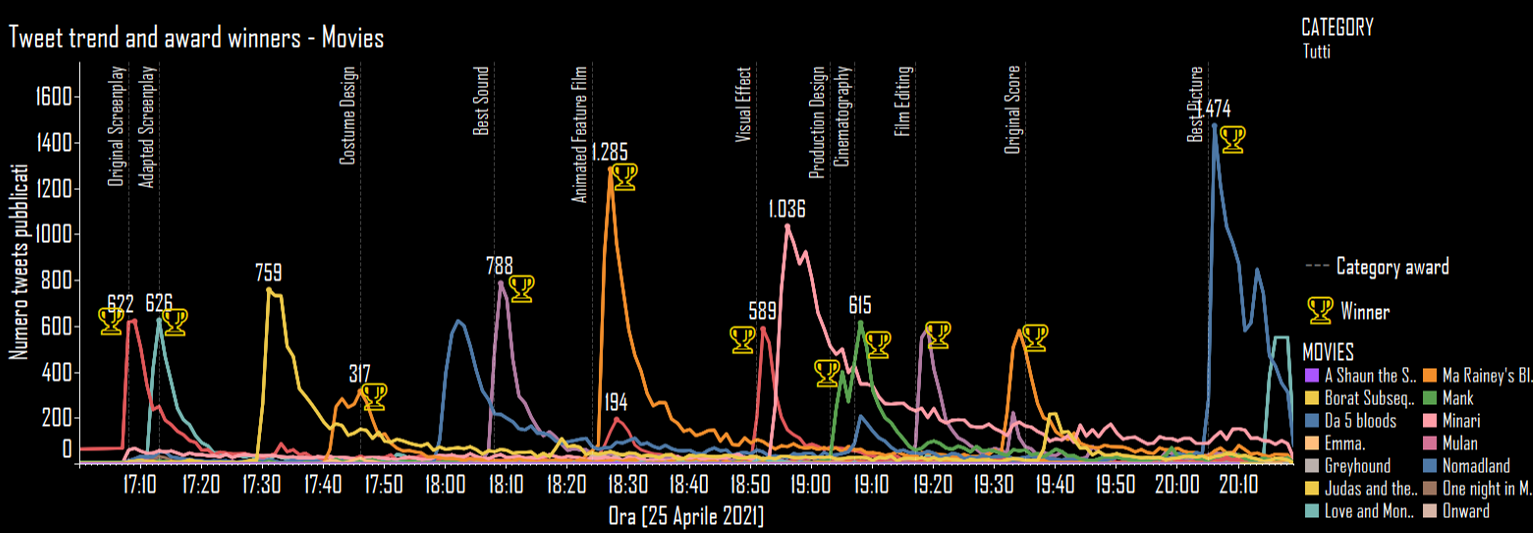
\includegraphics[width=1\linewidth]{imgs/INFOGRAFICA1.png}
			\caption{Prima Infografica}
			\label{fig:Prima infografica}
		\end{figure}


Nello specifico abbiamo raggruppato i film e gli attori per categorie a cui sono stati nominati. L'aggiunta delle linee tratteggiate che rappresentano il momento della premiazione permettono di avere una visione completa dell'evento. Al candidato vincitore è associata una coppa che indica la vittoria per la categoria specifica.

Per quanto concerne la domanda di ricerca possiamo affermare che esista una corrispondenza dei picchi con l'effettiva premiazione, ma sono visibili anche ulteriori picchi che apparentemente non sembrano avere corrispondenza. Confrontando la prima infografica con la seconda si evince che i picchi “anomali" nell'infografica relativa ai film corrispondono alle premiazioni degli attori e derivano dal fatto che insieme al nome dell'attore è stato tweettato anche il titolo del film associato. 

Merita un discorso a parte invece il picco delle 19:50 circa relativo a Glenn Close (seconda infografica). In quel momento della serata infatti si è verificato un siparietto comico che ha coinvolto l'attrice portando un focus del pubblico su tale avvenimento che ha quindi generato un incremento di tweet.

In generale quindi risulta esserci una certa aderenza tra chi vince l'Oscar e il “picco di discussione" avvenuto su Twitter; possiamo anche notare però quanto avvenuto nel caso di Anthony Hopkins che ha vinto il premio come “Best Actor" ed ha effettivamente ottenuto un picco a seguito della premiazione ma tale picco risulta estremamente inferiore rispetto agli altri, avvenimento che ci possiamo spiegare a seguito del fatto che la vincita dell'attore non è stata accompagnata da un gradimento da parte del pubblico.

\section{Rating (TMDB) vs count tweets - Movies \& Actors/Actress}

La terza e la quarta infografica consentono un confronto fra quanto è stato discusso un film (attore/attrice) e il punteggio ottenuto dalla critica (popolarità), tuttavia rispetto alle visualizzazioni precedenti i tweet sono stati raggruppati in fasce orarie (attraverso una aggregazione ogni 30 minuti).  La realizzazione di queste ultime ha permesso di rispondere alla seconda e alla terza domanda di ricerca: “I film che vincono l'Oscar sono anche quelli più acclamati dalla critica? Gli attori che prendono la famosa statuetta sono anche i più popolari?". 

	\begin{figure}[h]
			\centering
			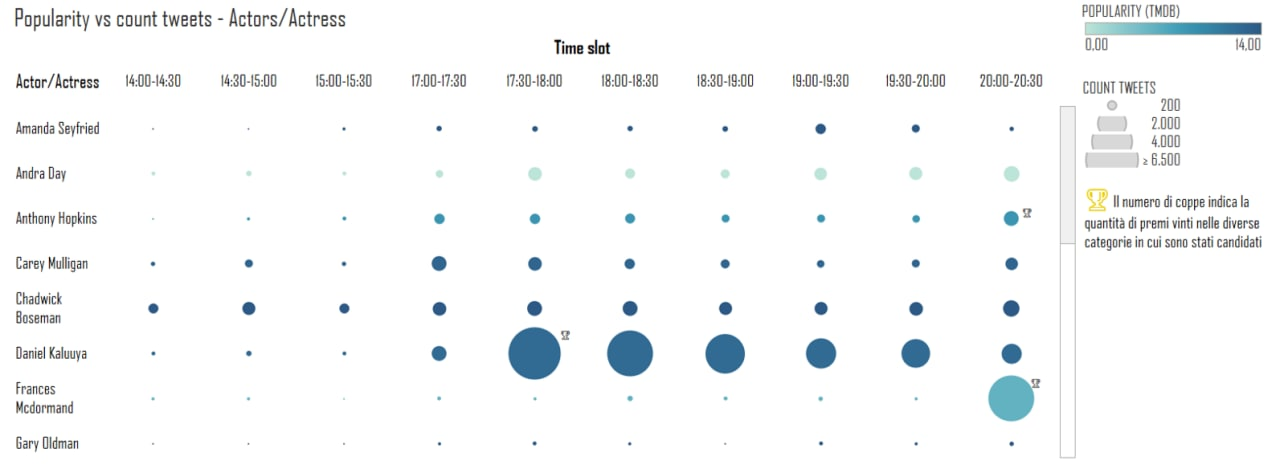
\includegraphics[width=1\linewidth]{imgs/photo1631116691.jpeg}
			\caption{Terza Infografica}
			\label{fig:Terza infografica}
		\end{figure}

  Per ciò che riguarda i film si nota una corrispondenza fra i film vincitori e un alto valore del rating, si vedano ad esempio i film Soul, The Father, Sound of Metal, Tenet. Un'eccezione è invece rappresentata dal film Wolkwalkers che pur ottenendo un rating pari a 8.5 non ha ottenuto alcun Oscar. Per ciò che concerne gli/le attori/attrici si nota una quasi totale corrispondenza tra vincita dell'Oscar e alti valori di dellla popolarità ad eccezione dell'attrice Yuh Jung Joun che non presentava alcun rating sulla piattaforma TMDB, va notato infatti che nonostante l'attrice avesse già partecipato a dei film per il mercato orientale, il film Minari ha sancito il suo debutto su quello occidentale.

\newpage
\section{Movies Categories \& Actors/Actress Categories}
Anche in questo caso sono state create due infografiche che andassero a mostrare a fine serata, quale è stata (o sono state) la categoria più discussa dal pubblico. In questo caso il trend dei tweet è stato costruito mediante un'aggregazione degli stessi per categoria. 

	\begin{figure}[h]
			\centering
			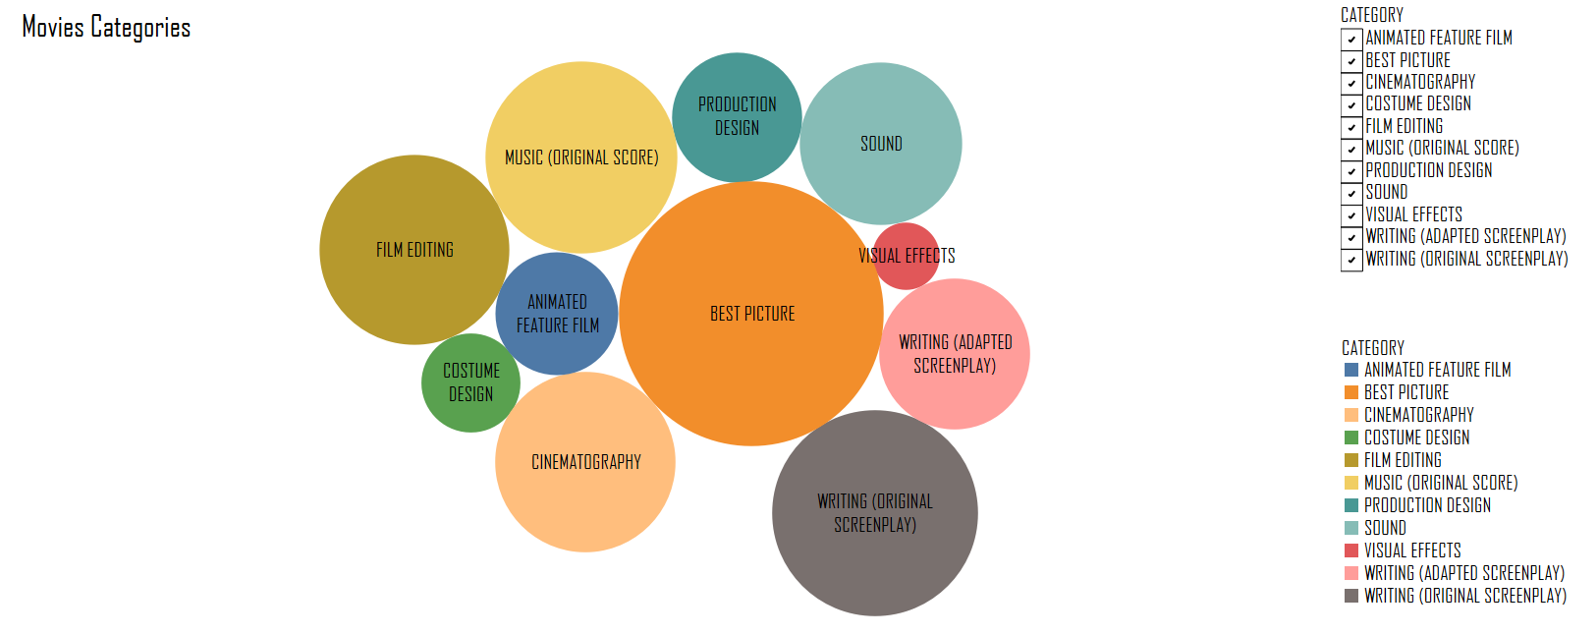
\includegraphics[width=1\linewidth]{imgs/Infografica5OKOK.png}
			\caption{Quinta Infografica}
			\label{fig:Terza infografica}
		\end{figure}
		
La quinta infografica mostra come la categoria più discussa relativa ai premi per i film sia “Best Picture", questo non sorprende in quanto questa categoria è la più ambita e importante.
La sesta infografica invece, ci permette di apprezzare un dato sorprendente: le categorie corrispondenti ai “supporting role" maschile e femminile sono stati maggiormente discussi rispetto ai “leading role", fatto interessante visto che il “supporting role" era storicamente considerato meno rilevante.
Infine, si nota anche che per quanto riguarda attori e attrici, queste ultime hanno raccolto un maggior numero di tweet rispetto agli attori.

\chapter{Valutazione della qualità}
Per la valutazione della qualità delle infografiche è stata svolta:
\begin{itemize}
 \item \textit{Valutazione euristica};
 \item \textit{Questionario psicometrico};
 \item \textit{User test}.
\end{itemize}

\section{Valutazione euristica}
La valutazione euristica è stata sottoposta a tre persone; i soggetti hanno potuto interagire liberamente con le visualizzazioni senza svolgere dei task specifici ma con la sola richiesta di parlare a voce alta in modo da capire quali fossero le difficoltà maggiori e se ci fossero incomprensioni. A seguito di tale test sono state modificate le infografiche così come sono visibili sopra. 

\subsection{Prima e seconda infografica}
La prima infografica appare un po' caotica quando vengono visualizzati tutti i film, questo è un problema che si  riscontra per via dei tanti film rappresentati in un'unica visualizzazione. Dopo un primo impatto però selezionando le categorie viene compresa meglio la visualizzazione e ciò che si vuole comunicare. Un altro problema riscontrato riguarda il fatto che la visualizzazione partiva da una categoria pre-selezionata, invece si preferisce che vengano visualizzati tutti gli andamenti per poi andare a filtrare man mano.

\subsection{Terza e quarta infografica}
Nella terza e quarta infografica si sono riscontrate difficoltà nel capire cosa sia “rating TMDB" (punteggio dato dalla critica ad ogni film) e nel capire da cosa è dato “popularity". 

\subsection{Quinta e sesta infografica}
Infine per la quinta e sesta infografica il soggetto ritiene più utile poter selezionare più categorie invece che una sola (quindi mettere un menù differente) in modo da poter effettuare confronti. 

\section{Questionario psicometrico}

Ad un campione di 20 soggetti è stato sottoposto un questionario psicometrico nel quale per le prime cinque infografiche sono state poste le seguenti domande: 

\begin{itemize}
    \item Quanto ritieni utile l'infografica ... ?
    \item Quanto ritieni intuitiva l'infografica ... ?
    \item Quanto ritieni chiara l'infografica ... ?
    \item Quanto ritieni informativa l'infografica ... ?
    \item Quanto ritieni bella l'infografica ... ?
    \item Come valuti complessivamente l'infografica ... ?
\end{itemize}

Non si è ritenuto importante sottoporre alla valutazione psicometrica la sesta infografica essendo molto simile alla quinta infografica. 

I risultati ottenuti sono stati sintetizzati grazie all'ausilio di grafici quali: Stacked barplot e Correlogramma.

\subsection{Prima e seconda infografica}

	\begin{figure}[h]
			\centering
			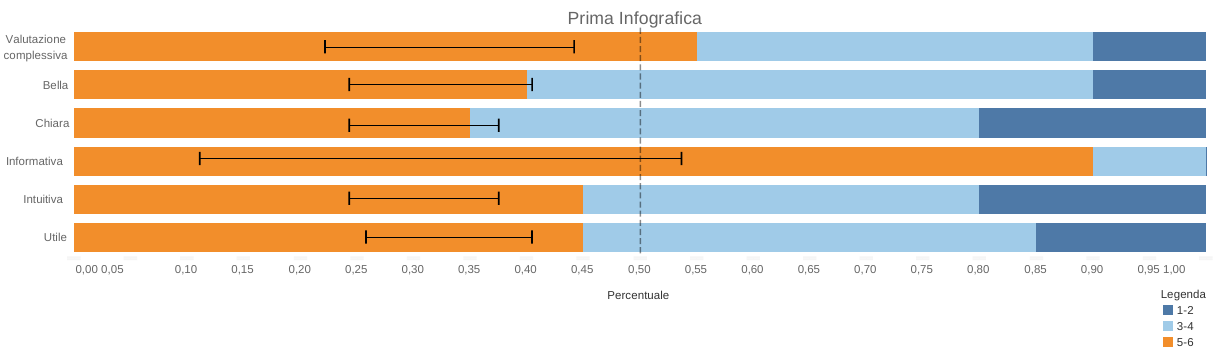
\includegraphics[width=1\linewidth]{imgs/vis1.png}
			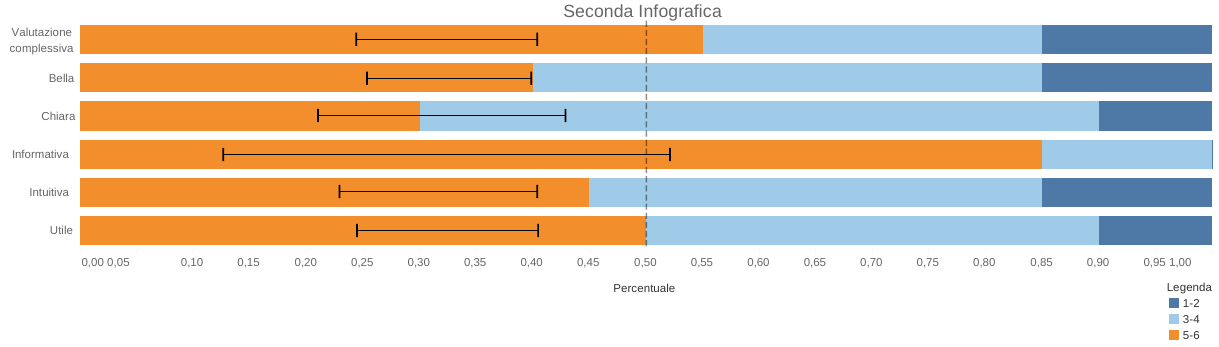
\includegraphics[width=1\linewidth]{imgs/vis2.png}
			\caption{Stacked barplot}
			\label{fig:Terza infografica1}
		\end{figure}
Gli stacked bar plot riferiti alle prime due infografiche mostrano risultati interessanti. Possiamo infatti notare come per entrambi l'intervallo di confidenza per la voce \textit{Informativa} includa il valore 0.5. Da ciò si può concludere che tale maggioranza non è significativa e pertanto non può rappresentare il giudizio dell'intera popolazione. Viceversa per la voce \textit{Valutazione Complessiva} il giudizio fornito dalla maggioranza risulta significativo quindi potrebbe essere rappresentativo dell'intera popolazione. 
\newpage

\begin{figure}[h]
			\centering
			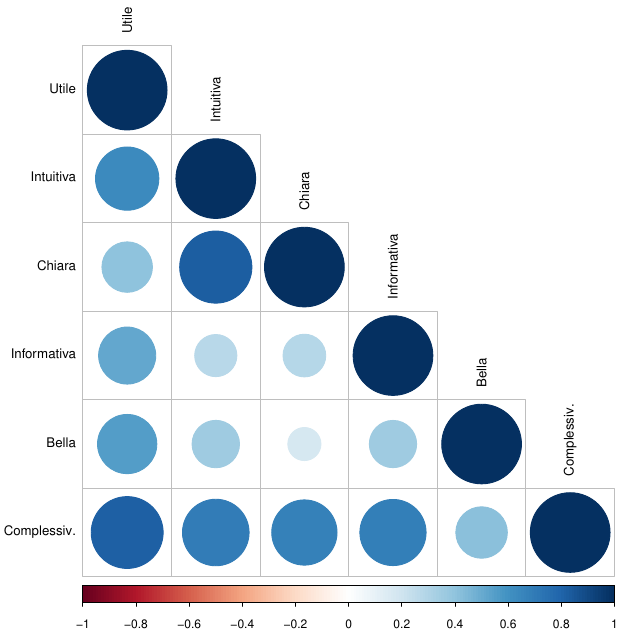
\includegraphics[width=0.4\linewidth]{imgs/corrVIS1.png}
			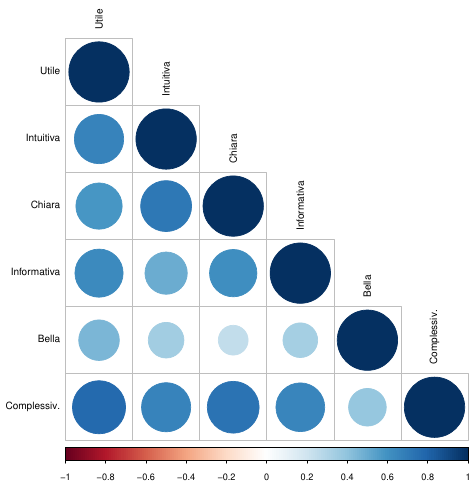
\includegraphics[width=0.4\linewidth]{imgs/corrVIS2.png}
			\caption{Correlogramma Prima Infografica (sx) e Seconda Infografica (dx)}
			\label{fig:Terza infografica1}
		\end{figure}
		

Dai correlogrammi si può invece notare un'alta correlazione fra le voci \textit{Intuitiva} e \textit{Chiara} e fra \textit{Complessiva} e \textit{Utile}, meno accentuata è invece la correlazione fra \textit{Intuitiva} e \textit{Utile} e fra \textit{Complessiva} e le voci: \textit{Intuitiva}, \textit{Chiara} e \textit{Informativa}. Molto bassa risulta inoltre la correlazione tra \textit{Bella} e le altre voci per entrambe le infografiche, sintomo del fatto che per queste due hanno prevalso altre qualità sulla bellezza come l'informatività e l'utilità.


\subsection{Terza e quarta infografica}

	\begin{figure}[h]
			\centering
			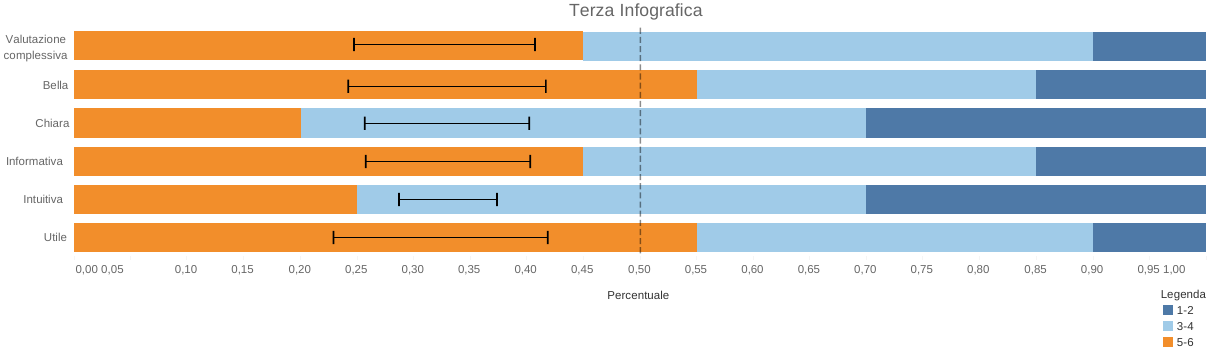
\includegraphics[width=1\linewidth]{imgs/vis3.png}
			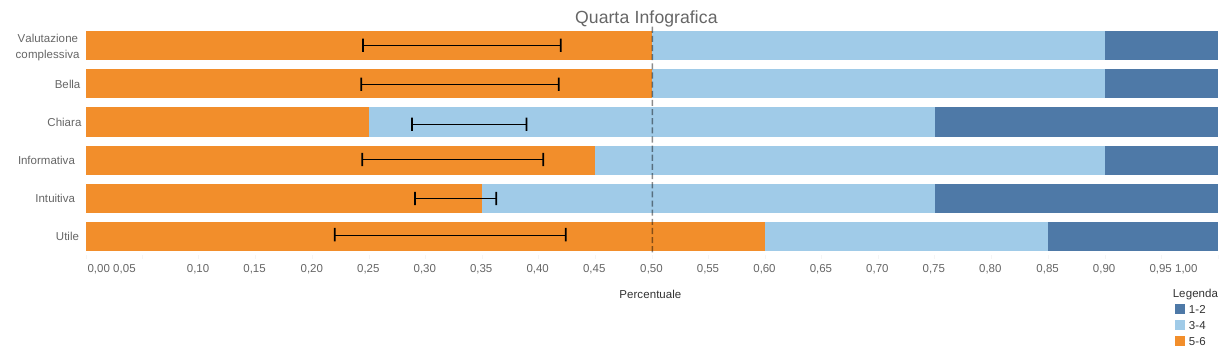
\includegraphics[width=1\linewidth]{imgs/vis4.png}
			\caption{Stacked barplot}
			\label{fig:Terza infografica11}
		\end{figure}

Gli stacked bar plot riferiti alla terza e quarta infografica mostrano invece la presenza di una maggioranza significativa rispettivamente per le voci \textit{Bella} e \textit{Utile} e per la voce \textit{Utile}.  

\begin{figure}[h]
			\centering
			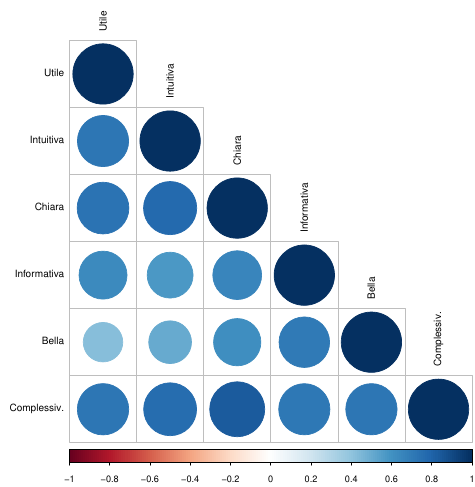
\includegraphics[width=0.4\linewidth]{imgs/corrVIS3.png}
			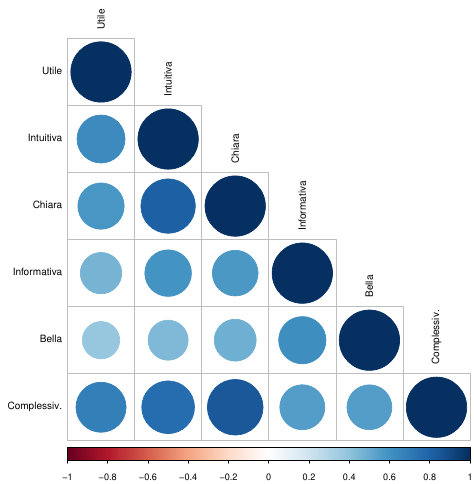
\includegraphics[width=0.4\linewidth]{imgs/corrVIS4.png}
			\caption{Correlogramma Terza Infografica (sx) e Quarta Infografica (dx)}
			\label{fig:Terza infografica111}
		\end{figure}

\newpage
Mentre dai correlogrammi si può notare che vi è un'alta correlazione fra la voce \textit{Complessivamente} e le voci \textit{Utile}, \textit{Intuitiva} e \textit{Chiara} e ancora fra \textit{Chiara} e \textit{Utile}, fra \textit{Chiara} e \textit{Intuitiva}. Per entrambe le infografiche risulta più debole la correlazione fra \textit{Bella} e \textit{Utile} e fra \textit{Bella} e \textit{Intuitiva}. Molto probabilmente per tali infografiche prevale la chiarezza, l'intuitività e l'utilità sulla bellezza. 

\subsection{Quinta infografica}

	\begin{figure}[h]
			\centering
			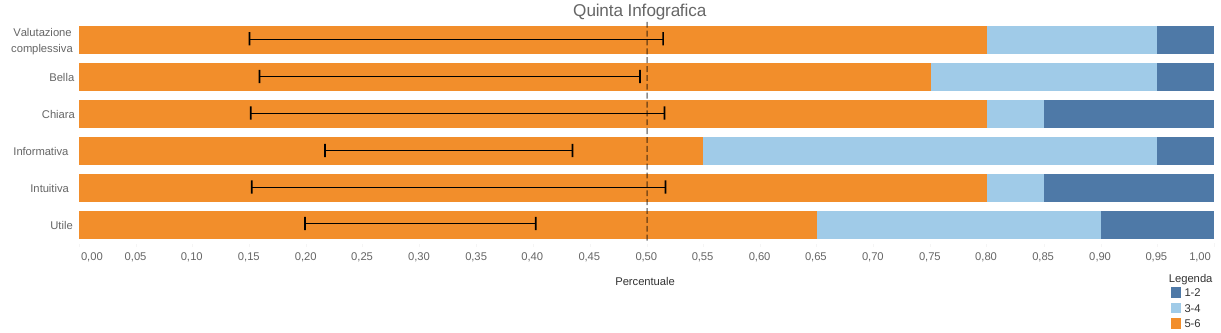
\includegraphics[width=1\linewidth]{imgs/vis5.png}
			\caption{Stacked barplot}
			\label{fig:Terza infografica11}
		\end{figure}
Infine per la quinta infografica, per le voci: \textit{Valutazione Complessiva}, \textit{Chiara} e \textit{Intuitiva} la maggioranza non risulta significativa, mentre risulta significativa la maggioranza relativa alle voci \textit{Bella}, \textit{Informativa} e \textit{Utile}. 	Rispetto alle infografiche precedenti questa viene ritenuta particolarmente bella e utile.  

\newpage

\begin{figure}[h]
			\centering
			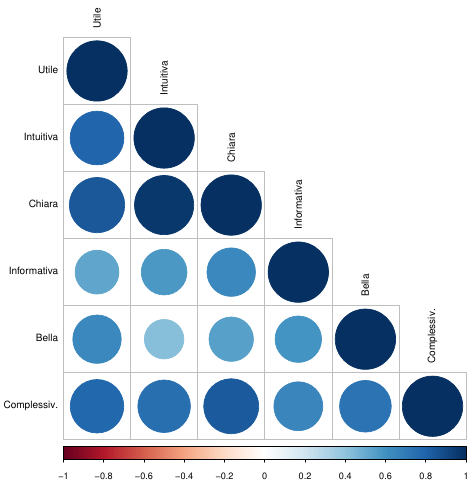
\includegraphics[width=0.4\linewidth]{imgs/corrVIS5.png}
			\caption{Correlogramma Quinta Infografica}
			\label{fig:Terza infografica111}
		\end{figure}


Nell'ultimo correlogramma è possibile notare un'altissima correlazione fra le voci \textit{Chiara} e \textit{Intuitiva}, ciò suggerisce che l'ultima visualizzazione è più intuitiva rispetto alle precedenti, dove infatti la correlazione rispetto alle stesse voci risultava inferiore. 

\newpage
\section{User test}

Ad un campione di 10 soggetti è stato richiesto di svolgere cinque task che prevedevano l'interazione con le infografiche tenendo conto del tempo impiegato per rispondere. Ciò è stato fatto al fine di comprendere se le informazioni che volevamo trasmettere tramite le infografiche erano facilmente comprensibili.

I cinque task che sono stati sottoposti sono i seguenti: 
\begin{enumerate}
    \item Nelll'infografica 1, a quale film è associato il picco più alto di tweet?
    \item Nell'infografica  1, quale film ha vinto nella categoria “Best Picture"? Nell'infografica  2 quale attore/attrice ha vinto nella categoria “Actress in a supporting role"?
    \item Nella infografica 3 quale film ha ottenuto un “Rating TMDB" maggiore?
\item Nella infografica 4 chi è stato più discusso durante la serata (ha ottenuto più tweet complessivamente)?
\item A quale categoria appartengono i film meno discussi durante la serata?
\end{enumerate}
\begin{figure}[h]
			\centering
			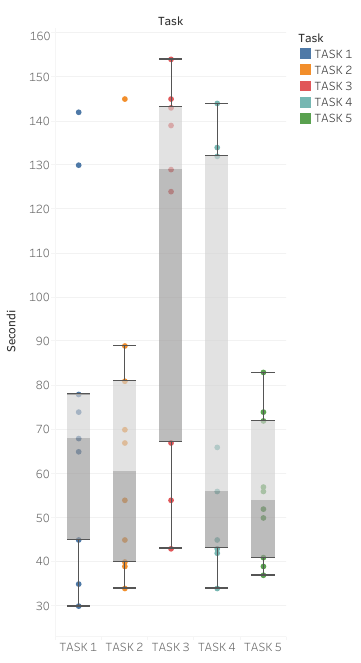
\includegraphics[width=0.4\linewidth]{imgs/User test.png}
			\caption{Box-plot user test}
			\label{fig:Terza infografica111}
		\end{figure}

Dal box-plot emerge che per task 1, 2 e 5 i tempi medi variano tra i 30 e i 90 secondi. Particolare invece risulta la situazione per i task 3 e 4 dove per il task 3 i tempi risultano visibilmente aumentati fino a superare i 120 secondi con la presenza di alcuni tempi molto bassi viceversa per il task 4 i tempi sono visibilmente bassi con la presenza di alcuni tempi molto alti.  

\paragraph{Link all'infografica}
\begin{verbatim}
https://public.tableau.com/views/DataVizProject_16311111989820/Storia1?
:language=it-IT&publish=yes&:display_count=n&:origin=viz_share_link
\end{verbatim}